\chapter{The game console}
\label{cha:GameConsole}

\section{Overview}
	\par The console has some specific features that will be described here. All of the aspects of hardware requirements, memory usage, input and output\ldots will be explained.
	Based on the image below, all requirements and specifications will be defined, from the controller to the interpreter to the graphics control.
	Any of these blocks is a stand-alone configuration, but the interpreter and the graphics control compose the actual console.

	\begin{figure}[H]
		\centering
		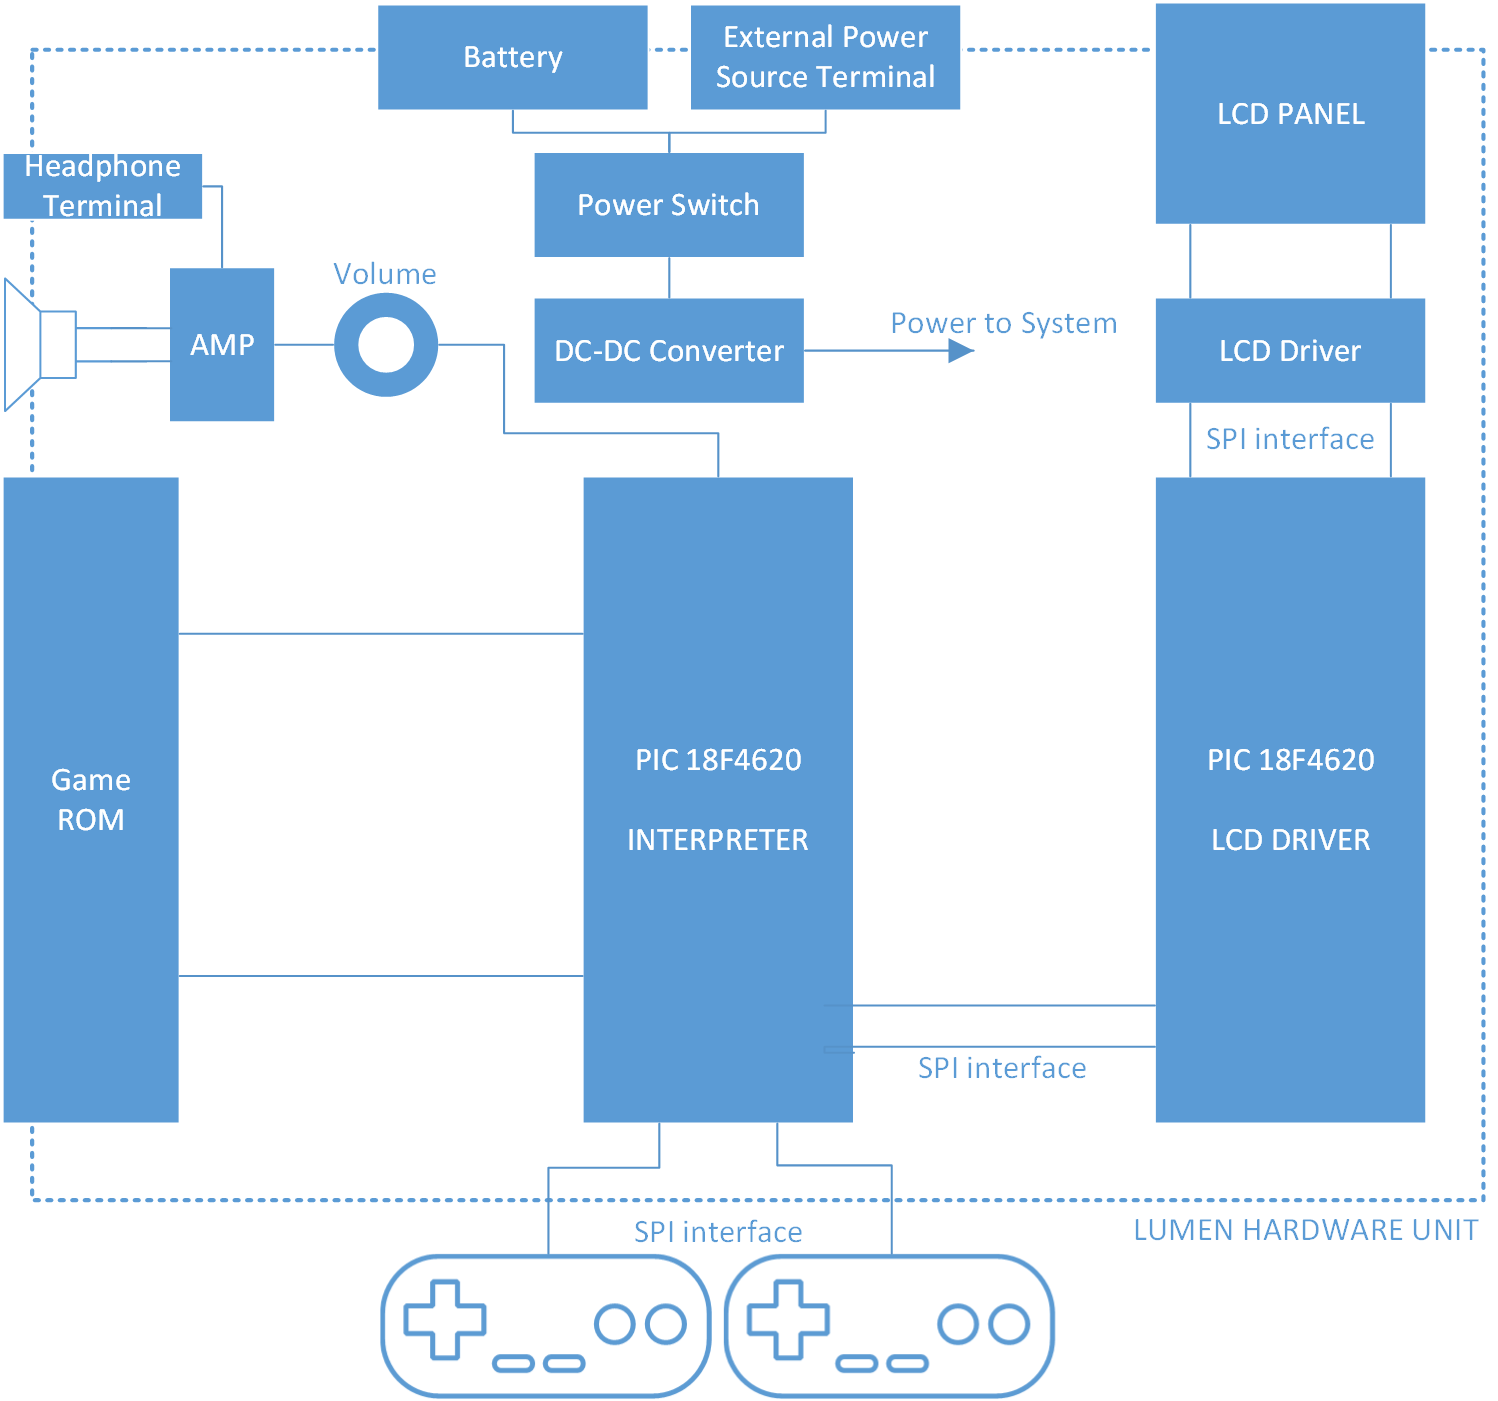
\includegraphics[width=0.9\textwidth]{GameConsole/LumenGameConsoleOverview.PNG}
		\caption{Console Overview}\par
		\label{fig:LumenGameConsoleOverview}
	\end{figure}

\newpage
\section{Controller}
	\subsection{Overview}
		\par A total of 8 push buttons are present on the controller, each with a pressed and a released state. When the user presses a button the state changes form released to pressed and vice versa. The controller uses an SPI interface to allow communication with the game.
		Multiplayer is possible when connecting 2 controllers at once.

		\begin{figure}[H]
			\centering
			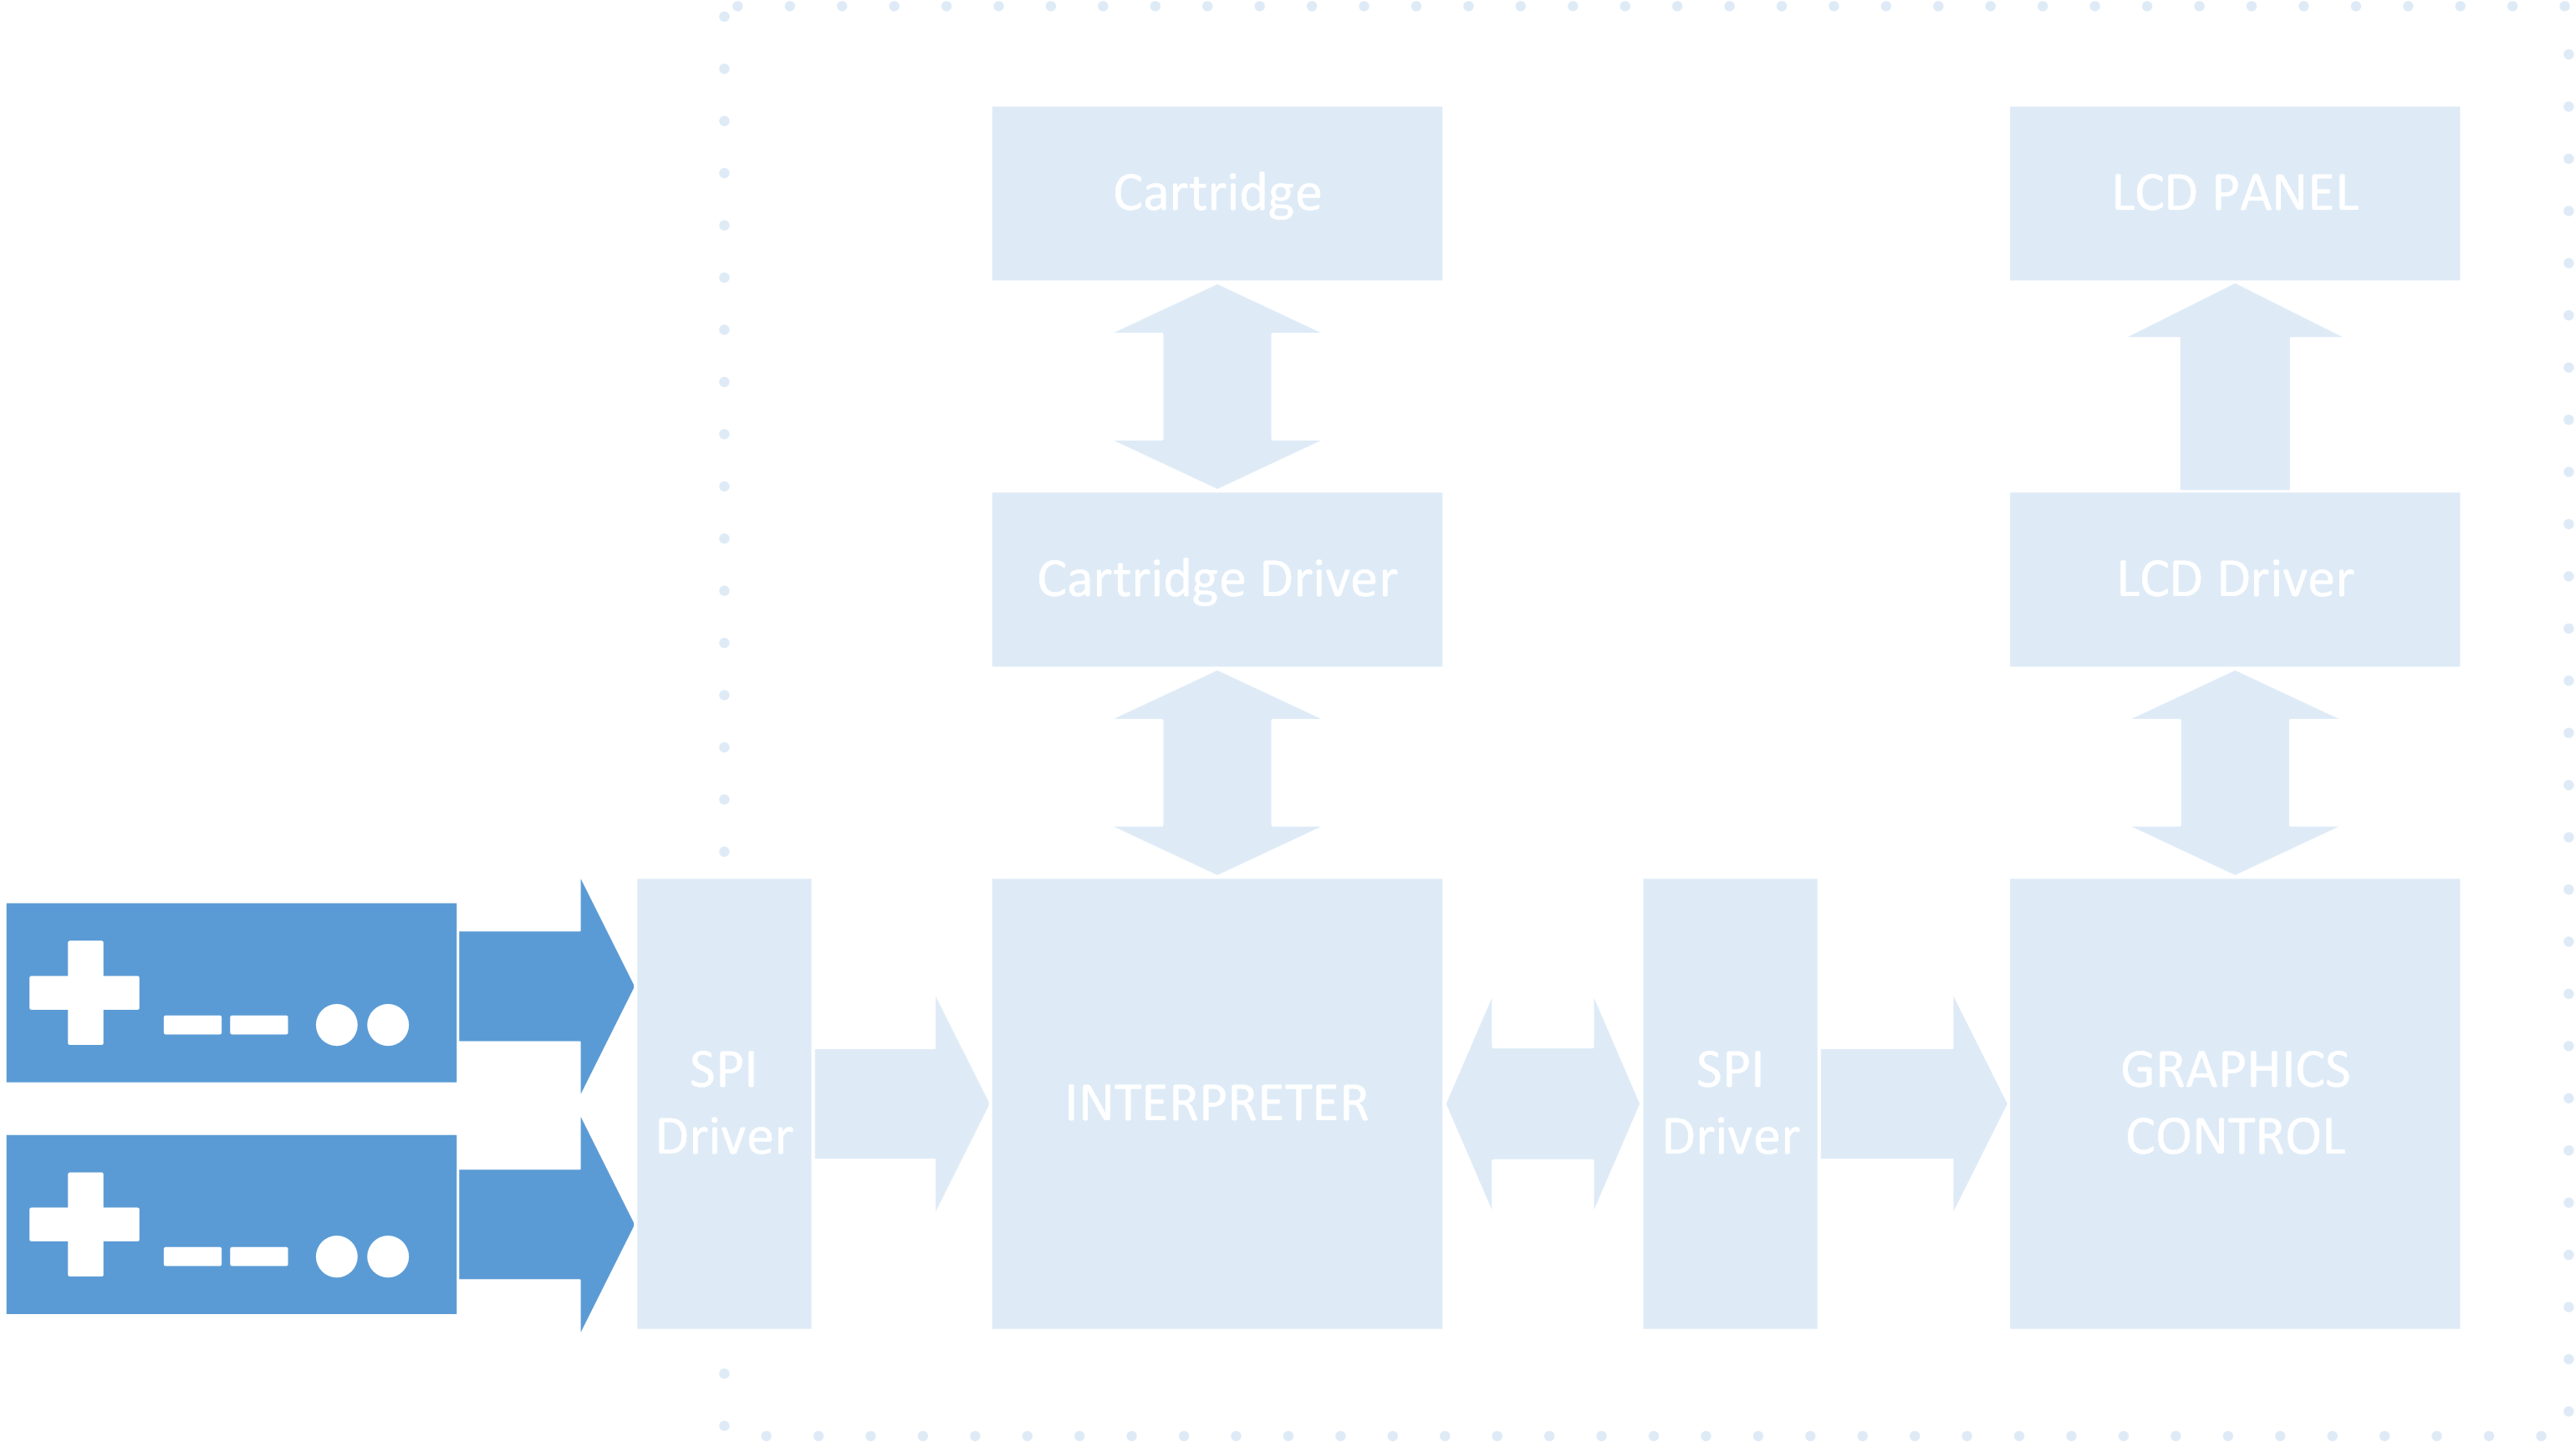
\includegraphics[width=0.4\textwidth]{GameConsole/Controllers_overview.PNG}
			\label{fig:ControllerOverview}
		\end{figure}

	\subsection{Buttons}
		\subsubsection{D-Pad}
			\par Four of the buttons at the left side of the controller are formed as a D-Pad, a flat thumb-operated four-way directional control with one push button on each point,
			providing intuitive direction and steering capabilities, and should be used as such.

		\subsubsection{Select and start}
			\par In the center, the select and start button are located.
			These should be used to start the game, pause it, allow menu navigation etc.
			The start button should allow pausing the game at any point, pressing start again returns to the game.

		\subsubsection{A and B}
			\par Next to the select and start buttons, A and B are located.
			These two buttons are to be used in-game, providing interaction with objects on the screen.
			They should not be used to pause or unpause the game at any time.

	\subsection{Interface}
		\par The controller connects through a three-wire interface similar to SPI. A maximum of two controllers can be connected, addressed as 0 and 1. The timing can be seen in this view (clockperiod of 6$\mu$s, from top to bottom: Latch, Clock, Data):

		\begin{figure}[H]
			\centering
			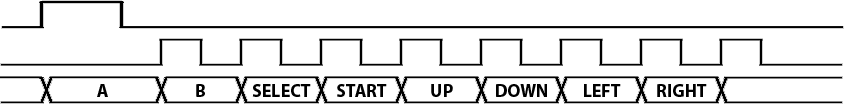
\includegraphics[width=0.7\textwidth]{GameController/ControllerInterface.PNG}
			\caption{Interface timing of the controller}\par
			\label{fig:ControllerInterface}
		\end{figure}

\section{Interpreter}
	\subsection{Overview}
		\par The interpreter is the main unit of the console. It executes the code and sends commands to the graphics controller to ensure the data displayed on screen is correct.
		Since the code is stored in external cartridge memory in the form of bytecode, specific requirement should be met to obtain accurate behaviour:
		\begin{itemize}
			\item MCU: PIC18F4620 (8-bit, 8 MHz)
			\item RAM: 3968 bytes - 256 bytes can be used by one game
			\item Input: NES controller (max 2)
		\end{itemize}

		\begin{figure}[H]
			\centering
			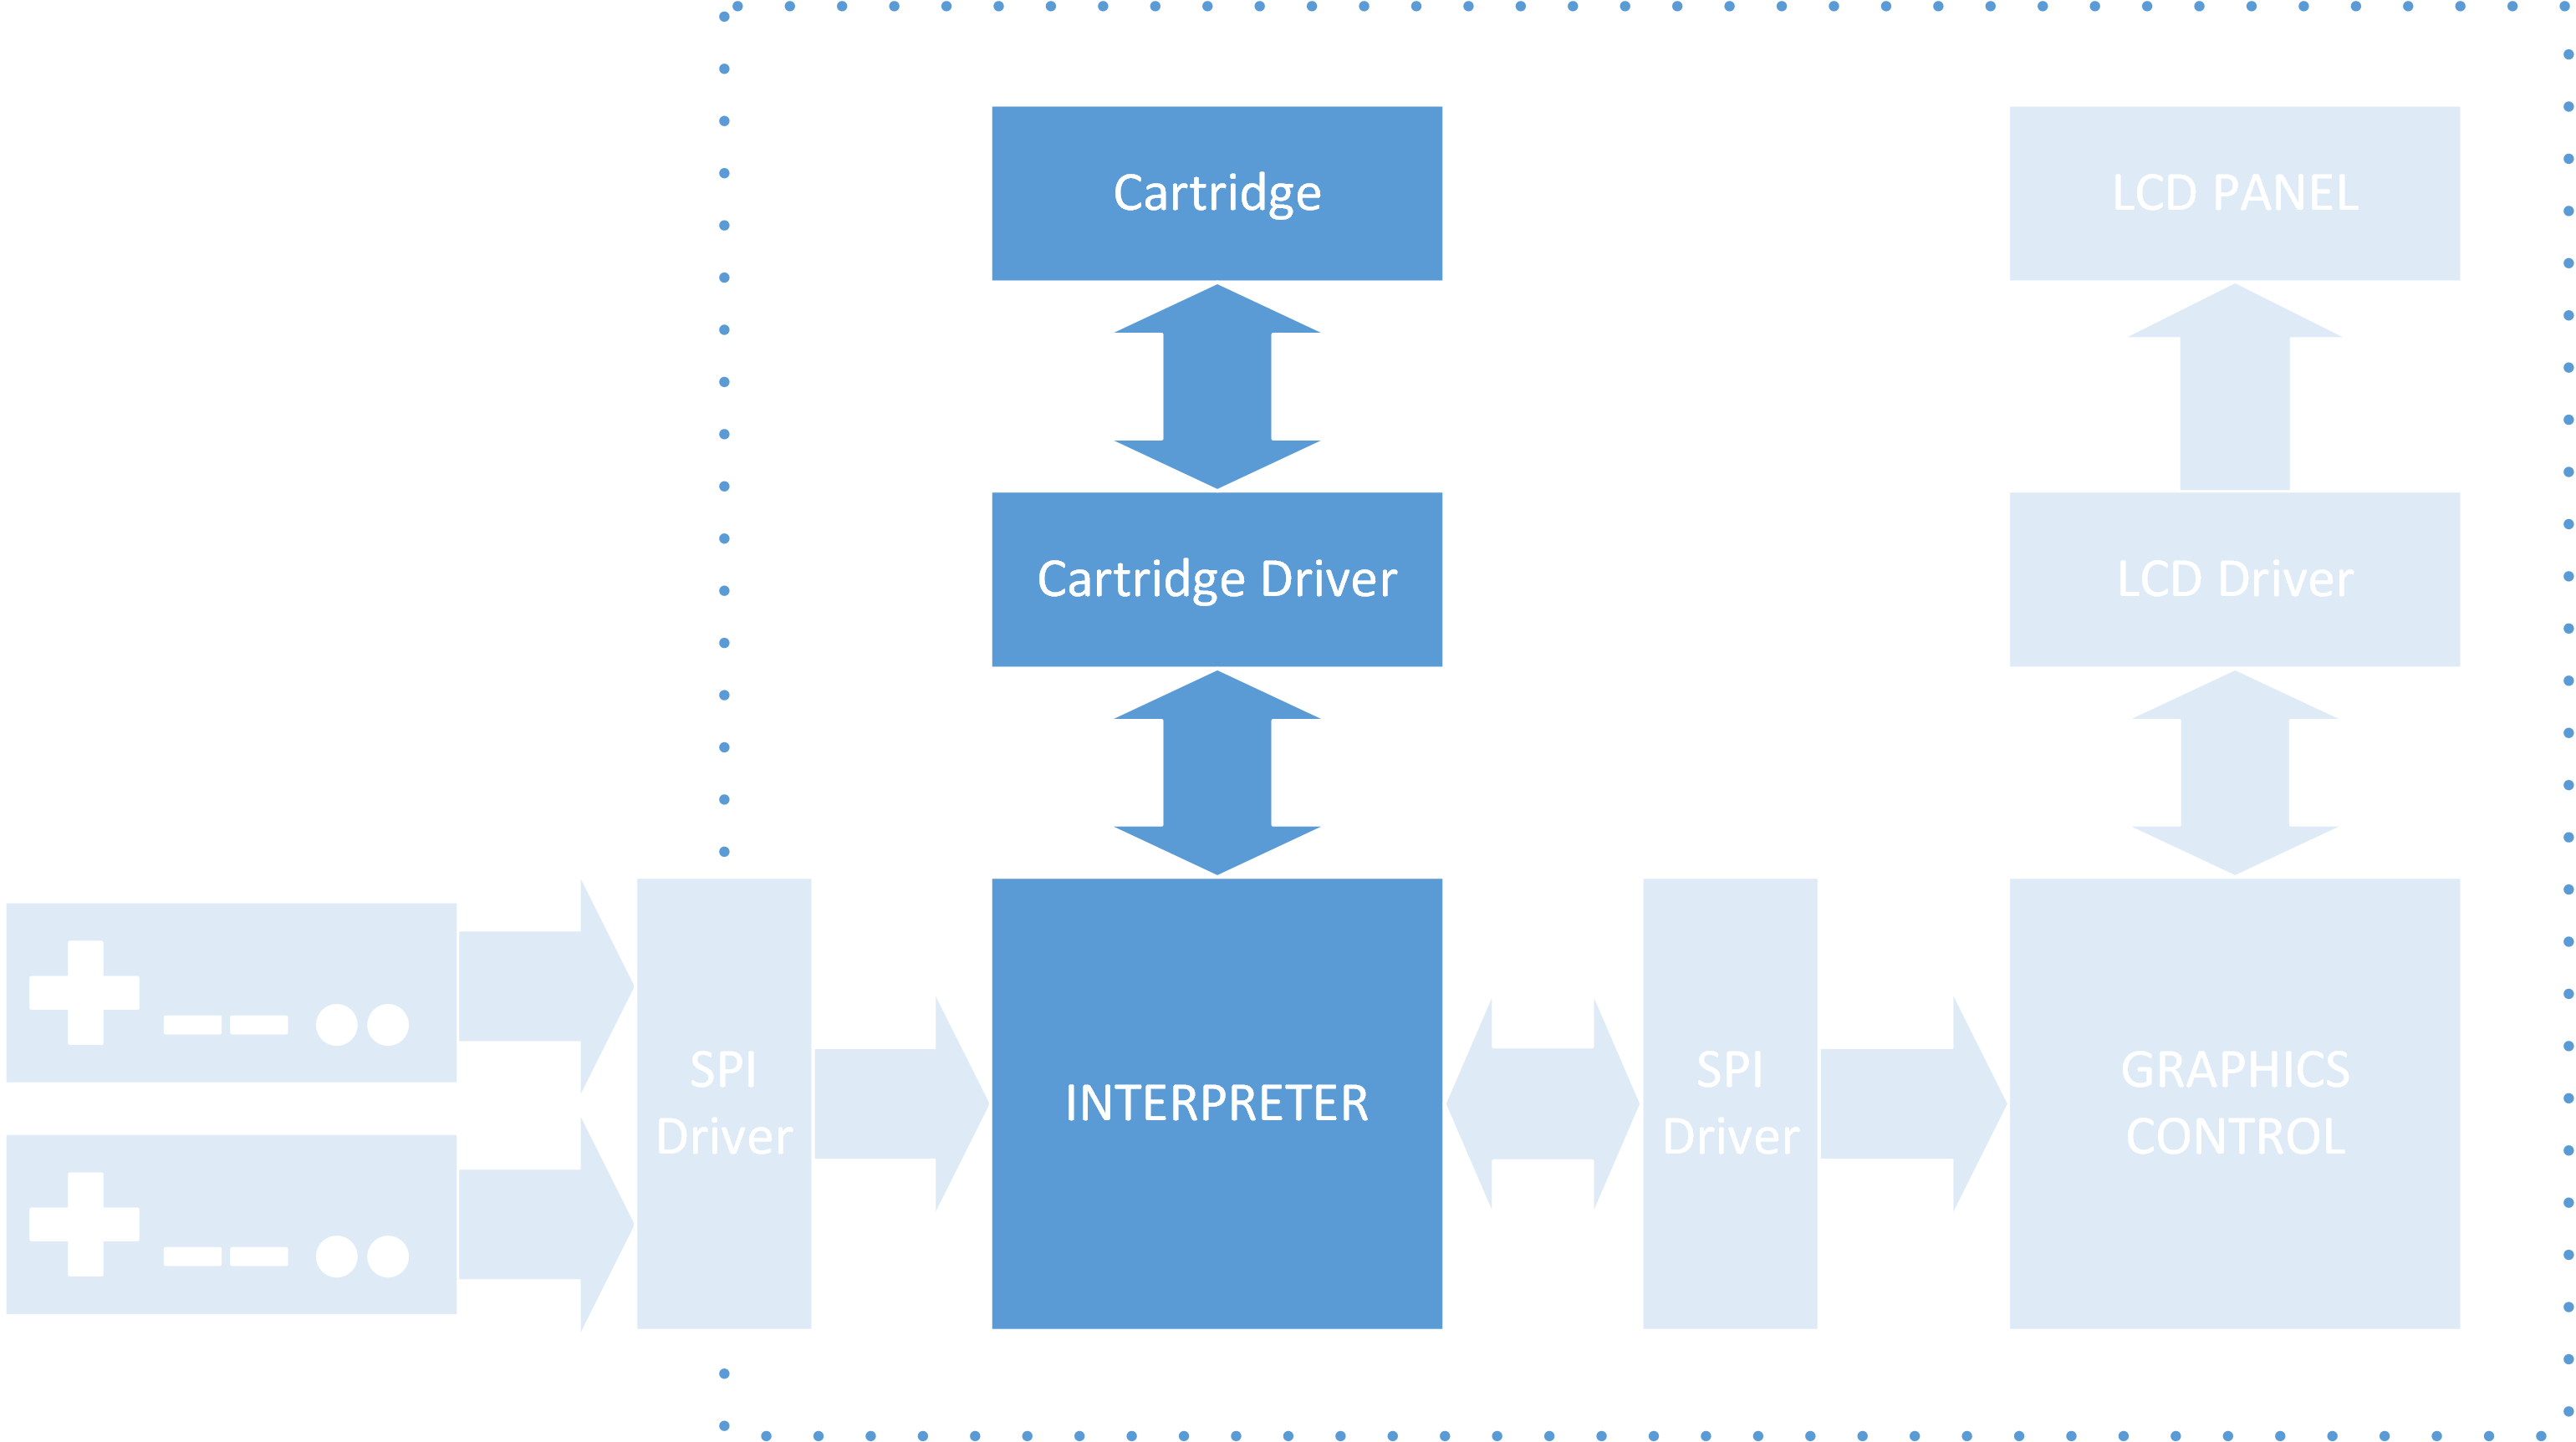
\includegraphics[width=0.4\textwidth]{GameConsole/Interpreter_overview.PNG}
			\label{fig:InterpreterOverview}
		\end{figure}

	\subsection{Peripherals}
		\subsubsection{Registers}
			\par Data transfer and manipulation is done via registers.
			These are memory locations that can be used to perform arithmetics on, used as delay counter\ldots
			They can be used as data storage, but the RAM is a better place for this.
			In total, 16 8-bit wide registers can be used, yet one should be used with caution since it will be overwritten by some specific instructions.
			Registers 0 to 14 are free to use, and will only be overwritten when the code tells the interpreter to do so.
			The 15th register, called the HL register, is used by the interpreter as data buffer for e.g. reading a controller or timer.

		\subsubsection{Stack}
			\par The stack is used to temporarly store data when the interpreter executes a subroutine or a register should be stored for later use.
			It is a LIFO structure of 256 items long, each item being 8 bit wide.
			The stack pointer is 8 bit too, but cannot be manipulated by the user directly: push and pop instructions are supported, and are available through the interpreter.

		\subsubsection{Program counter}
			\par The program counter is a pointer to where the interpreter is in the code.
			It is a 16 bit unsigned short, starting at 0 for the first instruction.
			Each instruction or operand increments this program counter.
			The program counter cannot be manipulated by the user directly, but should go through the jump, call or return instructions of the interpreter.
			A jump instruction replaces the program counter by a new value, while the call instruction pushes the current program counter to the stack and then replaces the program counter by the new one.
			Return pops the program counter from the stack at the end of a subroutine, and replaces the current program counter by this value, which results in a return to the point of calling the subroutine.

		\subsubsection{RAM}
			\par RAM can be used to store data during the execution of a program, it is 256 items long, each item being 8 bits wide.
			It will never be overwritten by the interpreter automatically, yet overwriting can happen when the code tells the interpreter to do so.
			It is possible to exchange data from a register to a RAM address and the other way around.
			Data that should be stored over a longer period of time can be placed in RAM, and copied back to a register for later manipulation.

	\subsection{Cartridge memory mapping}
		\par An important aspect of every game is the memory mapping on the cartridge.
		Every item (code, sprites, strings and maps) has its own specific start- and endaddress to establish a solid and correct performance. The mapping is as follows:

		\begin{figure}[H]
			\centering
			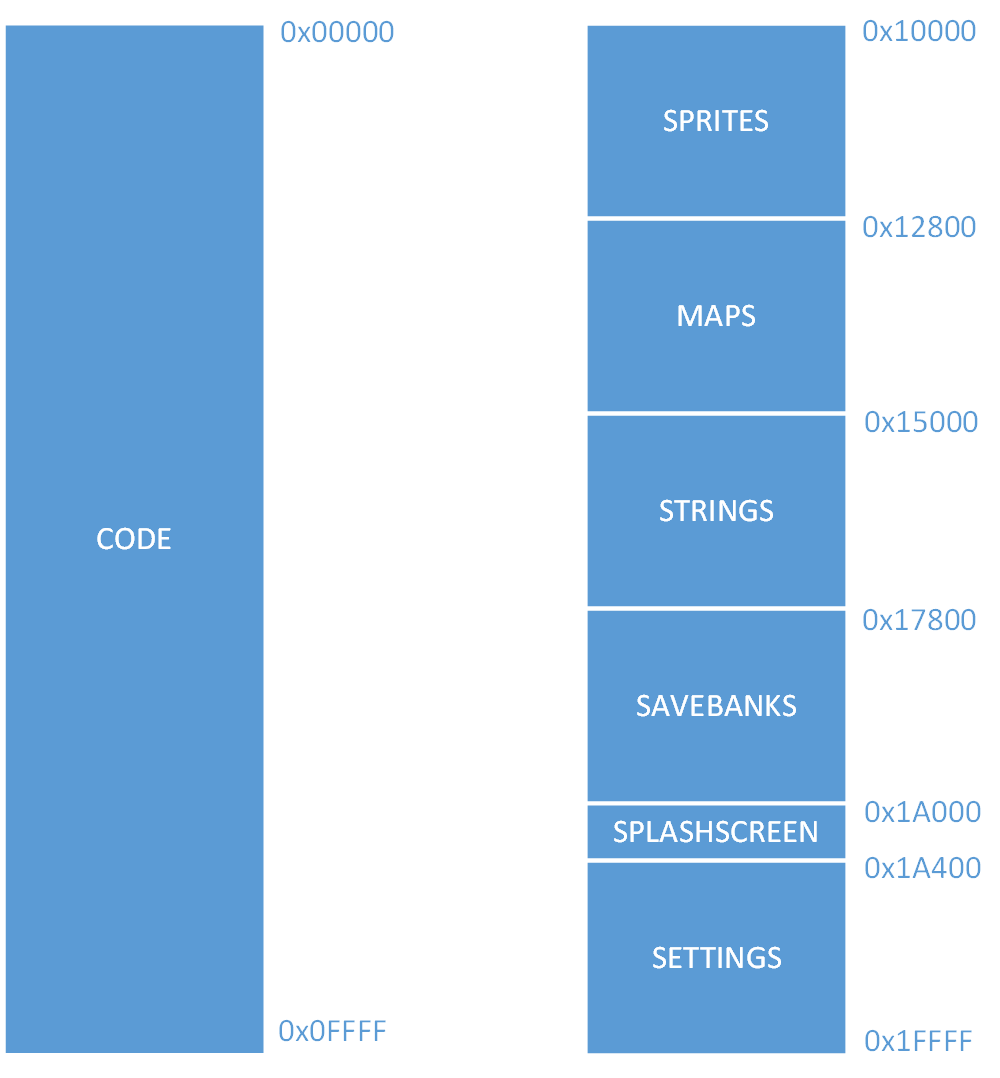
\includegraphics[width=0.65\textwidth]{GameConsole/MemoryMap.PNG}
			\caption{Memory map of the cartridge}\par
			\label{fig:MemoryMap}
		\end{figure}

		\subsubsection{Code}
			\par This is the actual bytecode that will be interpreted and executed. An in-depth look on the instructionset can be found in chapter~\ref{cha:InstructionSet}. The maximum codesize is 64kB, or 65536 bytes. If no jump is performed at byte 65535, the program counter will overflow, resulting in a reset of the program counter to zero. Code examples can be found in the appendix.

		\subsubsection{Sprites}
		\label{subsec:sprites}
			\par A sprite is an 8 by 8 pixels bitmap in black and white. Each bit represents one pixel, resulting in a size of 8 bytes per sprite.
			The addressing starts at the top left, and goes down per colum, this happens to be 8 bits, and can thus be packed in one byte.
			The first colum is the first byte, the second colum the second byte\ldots

			\begin{table}[h]
			\centering
				\begin{tabular}{m{0.2em} m{0.2em} m{0.2em} m{0.2em} m{0.2em} m{0.2em} m{0.2em} m{0.2em} cccccccccc}
					$\square$      & $\square$      & $\blacksquare$ & $\blacksquare$ & $\blacksquare$ & $\blacksquare$ & $\square$      & $\square$      &&& 0 & 0 & 1 & 1 & 1 & 1 & 0 & 0 \\
					$\square$      & $\blacksquare$ & $\square$      & $\square$      & $\blacksquare$ & $\blacksquare$ & $\blacksquare$ & $\square$      &&& 0 & 1 & 0 & 0 & 1 & 1 & 1 & 0 \\
					$\blacksquare$ & $\square$      & $\square$      & $\blacksquare$ & $\blacksquare$ & $\blacksquare$ & $\blacksquare$ & $\blacksquare$ &&& 1 & 0 & 0 & 1 & 1 & 1 & 1 & 1 \\
					$\blacksquare$ & $\square$      & $\blacksquare$ & $\blacksquare$ & $\blacksquare$ & $\blacksquare$ & $\blacksquare$ & $\blacksquare$ &&& 1 & 0 & 1 & 1 & 1 & 1 & 1 & 1 \\
					$\blacksquare$ & $\blacksquare$ & $\blacksquare$ & $\blacksquare$ & $\blacksquare$ & $\blacksquare$ & $\blacksquare$ & $\blacksquare$ &&& 1 & 1 & 1 & 1 & 1 & 1 & 1 & 1 \\
					$\blacksquare$ & $\blacksquare$ & $\blacksquare$ & $\blacksquare$ & $\blacksquare$ & $\blacksquare$ & $\blacksquare$ & $\blacksquare$ &&& 1 & 1 & 1 & 1 & 1 & 1 & 1 & 1 \\
					$\square$      & $\blacksquare$ & $\blacksquare$ & $\blacksquare$ & $\blacksquare$ & $\blacksquare$ & $\blacksquare$ & $\square$      &&& 0 & 1 & 1 & 1 & 1 & 1 & 1 & 0 \\
					$\square$      & $\square$      & $\blacksquare$ & $\blacksquare$ & $\blacksquare$ & $\blacksquare$ & $\square$      & $\square$      &&& 0 & 0 & 1 & 1 & 1 & 1 & 0 & 0 \\
				\end{tabular}
			\end{table}
			
			This sprite, representing a ball, has the binary representation in the right table.
			Since we address by colum, the first byte is 0b00111100, which corresponds to 0x3C.
			The second colum is 0b01001110, and thus 0x4E.
			When all pixels are calculated the bytes are placed after one another, resulting in a complete sprite, here 0x3C4E9FBFFFFF7E3C.

		\subsubsection{Maps}
			\par A map is a combination of sprites that can fill the background of the screen.
			Placing a map on the screen can be functional, e.g. in a platformer game, or aesthetically.
			It is in fact a tiled field containing the indexes of sprites in the onscreen memory, each tile being 8 by 8 pixels (equal to 1 sprite).
			For more information on maps, please refer to the chapter~\ref{subsec:maps}.

		\subsubsection{Strings}
			\par Strings can be used to be drawn on screen as guidelines or instructions to the user.
			They are to be stored in the cartrigde memory as null-terminated ascii encoded strings, and will be read as such.
			If a string is not null-terminated, the interpreter will read until the first null is encountered, which can result in unexpected behaviour.
			A maximun total size of 10kB of strings can be loaded into the ROM, yet that amount can never be displayed at once on the screen, since the string buffer is limited to 256 bytes.
			For more information on strings, refer to the chapters~\ref{subsec:stringdata} and ~\ref{subsec:strings}.

		\subsubsection{Savebanks}
			\par The savebanks are 10 address locations of each 1kB that can be used freely by the game.
			If playernames, highscores, achievements\ldots should be stored, this is the location to do so.
			The game will not check if the data is legitimate or not, this is up to the programmer.
			Settings should not be stored in savebanks, for this has its own address location.

		\subsubsection{Splash screen}
			\par A splash screen is the screen that should be shown while all data is loaded and transfered between the interpreter and the graphics control.
			It has to be a black and white bitmap addressed from the top left down each colum.
			Since the screen is 84x48, a fullscreen bitmap is 4032 bits, or 504 bytes.

		\subsubsection{Settings}
			\par Settings can be stored in this address location.
			No restrictions are applied, and the content is up to the programmer.

\section{Graphics control}

	\begin{figure}[H]
		\centering
		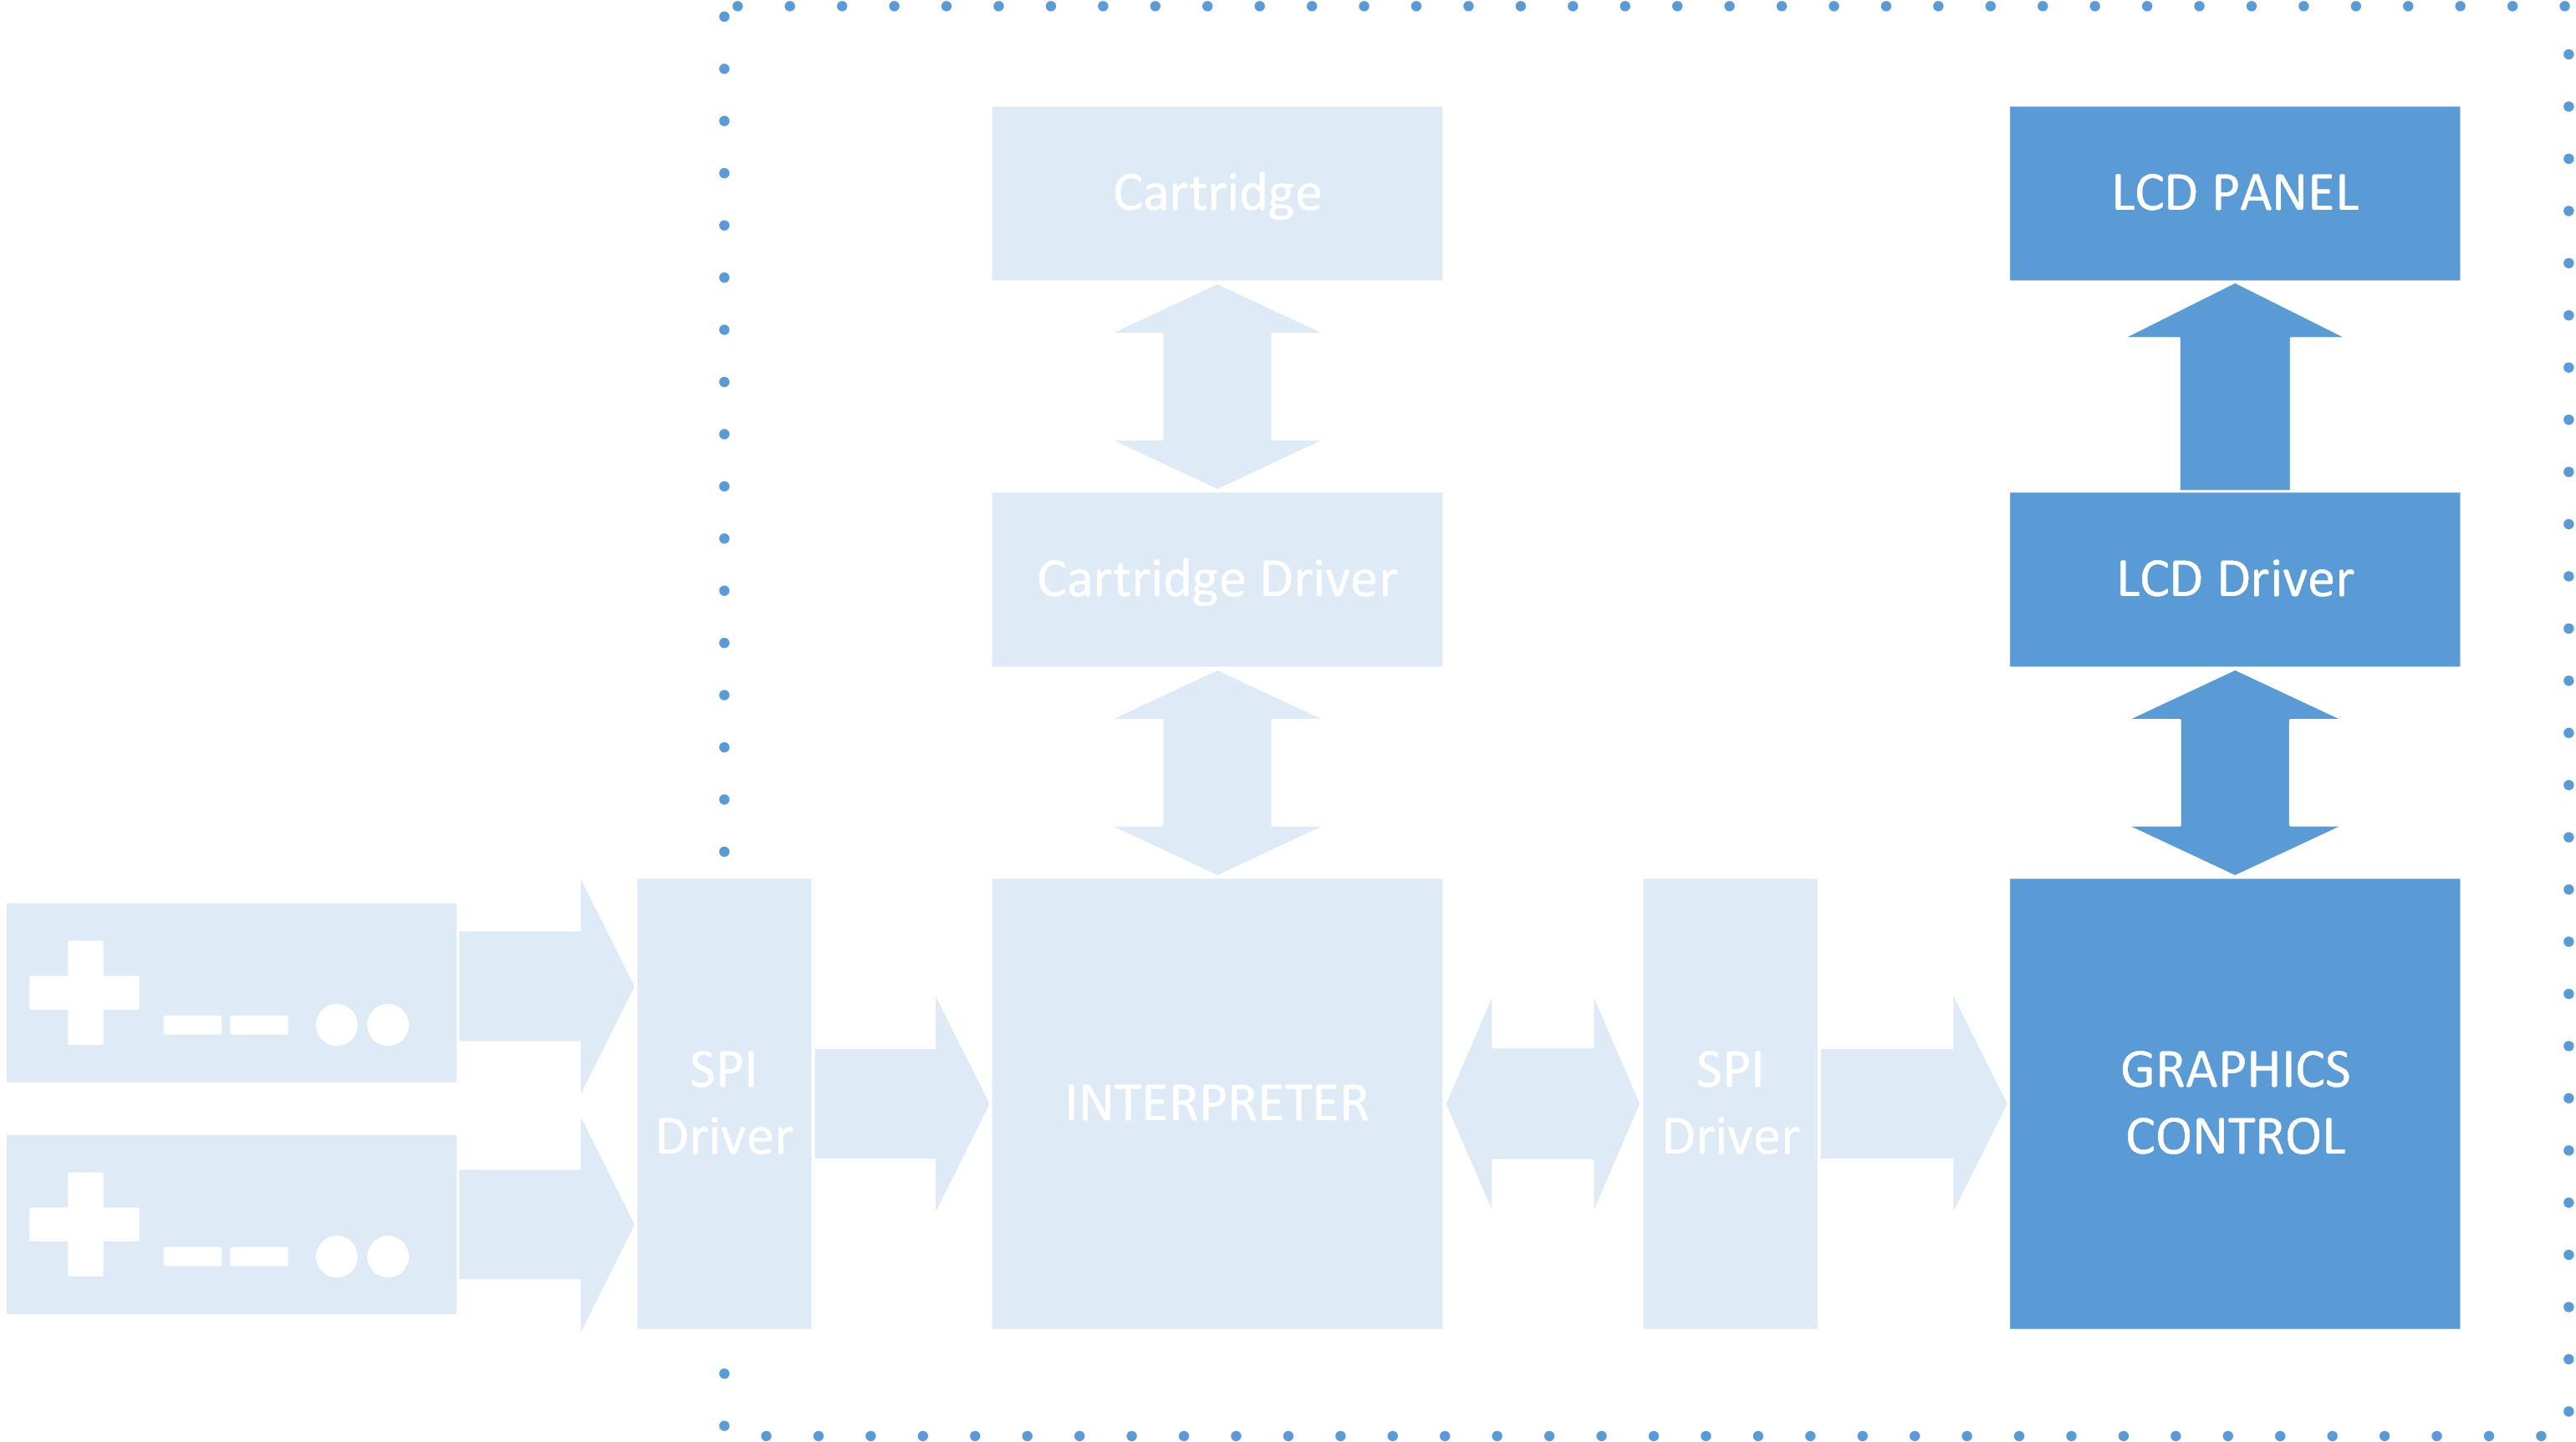
\includegraphics[width=0.4\textwidth]{GameConsole/GraphicsControl_overview.PNG}
		\label{fig:GraphicsControlOverview}
	\end{figure}

\chapter{The graphics control}
\label{cha:GraphicsControl}

\section{Overview}
	\par The graphics control is located entirely in a separate microcontroller. Its tasks in a nutshell are to drive the actual LCD display and to provide a simple way of using graphics in a game. To do so it provides a set of commands to the programmer that can be used to initialize, draw, move and remove spites on the screen. It also has support for text on screen and for maps that can be scrolled over the screen.

\section{The LCD display}
	\par The LCD display used in this setup has a resolution of 84x48 pixels. It has a PCD8544 chipset and is interfaced with SPI. The chipset does all the timing and scanning of the LCD. All we need to provide is a correct initialisation, fill the VRAM and send valid commands. This is where graphics control comes in. The graphics control translates SPI commands and data from the interpreter to SPI commands and data the LCD understands.

\section{Memories of the graphics control}
	\par The graphics control has several sort of memories. Although most of it is directly in ram, their purposes are completely different:

	\subsection{Sprites in memory}
		\par This part of the memory is used to store the actual data of a sprite, or the data for the visual representation of that particular sprite. It can contain up to 32 different sprites and a sprite is 8 by 8 pixels or 8 bytes in size. For an in-depth look on the format of sprites, please refer to chapter~\ref{subsec:sprites}.

		\par Every sprite in memory can be referenced by its number in memory, as there are 32 possible sprites valid numbers are from 1 up to 32.

	\subsection{Sprites on screen}
		\par This part of the memory tell the graphics control what to draw where concerning sprites. It can contain up to 32 record. A record is 3 bytes big and represents a sprite (first byte), a X position on the screen (second byte) and a Y position on the screen (third byte). From now on a sprite can be drawn on the screen. And a sprite on the screen is referenced by a list number, that number is the number of the record containing information of the sprite data and position. Note that multiple records can use the same sprite.

	\subsection{Maps}
	\label{subsec:maps}
		\par This part of the memory is used for background maps. Up to four maps can be used. A map exists of tiles and these tiles are in fact just sprites. One must use the the number of the spite in memory to use it in a map. A map measures 16 by 8 tiles, or 128 by 64 pixels. For tiling the map a sequence of references to sprites is needed. A map is tiled from left to right and than from top to bottom. When drawing a map on the screen, one can give a X and Y offset, resulting in a scrollable background.

	\subsection{Strings}
	\label{subsec:strings}
		\par This part of the memory is used to store pointers to string data. A string starts at the pointer location and ends when a null character is encountered. A maximum of 32 strings is allowed. The number of the string is used for referencing when drawing it to the screen.

	\subsection{String data}
	\label{subsec:stringdata}
		\par This part of the memory is used to store the actual data for the strings. It can contain up to 256 characters. Therefore all the strings (including null characters) together can have a maximum size of 256 bytes. A new string starts where the old string ended. Therefore it is important to initialize the strings at the beginning. Otherwise conflicts of overwriting strings is a ever present danger.

	\subsection{Font}
		\par This part of the memory contains the data for the actual graphical representation of a ascii character on the screen. A character is made of five bytes, and is mapped onto a 5x7 font. This part is also the only part not in RAM, it is hard coded in the flash region of the microcontroller.

	\subsection{VRAM}
		\par This part of the memory is of uttermost importance, this is where everything containing some graphic content different from text is drawn. It is used as sort of double buffer. In this part of the memory the final image is rendered. First the background map is drawn onto it, if needed. Then the sprites are drawn onto it. Once a full image is complete it is send to the LCD where it remains in its VRAM until a new image is send.

	\subsection{TRAM}
		\par This part of the memory is used to display text on the screen. To show text on the screen the graphics control receives numbers corresponding to the ascii standard. These numbers are converted to graphical data trough the font memory. When sending the image to the screen, the text data is combined with the graphics data by means of a XOR operation. So the text is black on a white background and white on a black background.
\section{The normal operation}
	\par The normal way to go is to initialize the graphics control using its provided initializer. This takes care of correct reset timings for the LCD. From then on the graphics control is ready to receive data. This data is received over SPI and the data received will be seen as a command followed by some arguments if necessary. Correct operation is not guaranteed when synchronisation is lost or when faulty commands are send. Correct commands are:
	\begin{tabular}{r|l}
		Command & Description \\
		Load sprite: 0x10 & Load a sprite in sprite memory \\
		Load map: 0x12 & Load a map in map memory \\
		Load string: 0x14 & Load a string in string memory \\
		Set sprite: 0x16 & Initialize a sprite in sprites on screen memory \\
		Update sprite: 0x18 & Draw a sprite on the screen at a certain position \\
		Clear sprite: 0x1A & Remove a sprite from the screen \\
		Draw map: 0x1C & Draw a map on the screen with a certain offset \\
		Draw string: 0x1E & Draw a string on the screen at a certain position \\
		Clear all: 0x20 & Clear both VRAM and TRAM \\
		Clear graphics: 0x22 & Clear VRAM \\
		Clear strings: 0x24 & Clear TRAM \\
		Redraw: 0x26 & Send the VRAM and TRAM to the LCD \\
		All on: 0x28 & Turn all the pixels on, draw them all black \\
		All off: 0x2A &  Turn all the pixels of, draw them white\\
		Invert: 0x2C &  Enable the inverted mode, black is white and vice versa\\
		Normal: 0x2E &  Enable normal mode, to restore from inverted mode\\
	\end{tabular}
	The reception of SPI communication is done in the background by interrupts. In the foreground a routine constantly checks for new commands. If a command is received the routine waits for the needed arguments, and then it calls the corresponding function.



